\documentclass{article}
\usepackage[english]{babel}
\usepackage[letterpaper,top=2cm,bottom=2cm,left=2.5cm,right=2.5cm,marginparwidth=1.25cm]{geometry}

\usepackage{hyperref, booktabs, float}
\usepackage[leqno]{amsmath}
\usepackage{enumitem, nccmath,lipsum,amssymb,xcolor,xparse,listings, blindtext}
\usepackage[most]{tcolorbox}

\usepackage{graphicx}
\graphicspath{ {./attachments/} }

\NewDocumentCommand{\codeword}{v}{\texttt{\textcolor{blue}{#1}}}

\lstset{language=C, keywordstyle={\bfseries \color{blue}}}

\NewDocumentCommand{\mynote}{+O{}+m}{%
  \begingroup
  \tcbset{%
    noteshift/.store in=\mynote@shift,
    noteshift=1.5cm
  }
  \begin{tcolorbox}[nobeforeafter,
    enhanced,
    sharp corners,
    toprule=0.5pt,
    bottomrule=0.5pt,
    leftrule=0pt,
    rightrule=0pt,
    colback=green!10,
    #1,
    left skip=\mynote@shift,
    right skip=\mynote@shift,
    overlay={\node[right] (mynotenode) at ([xshift=-\mynote@shift]frame.west) {\textbf{Note:}} ;},
    ]
    #2
  \end{tcolorbox}
  \endgroup
  }
\makeatother

\newcommand{\mytext}[1]% #1 = same as intertext
{&\parbox{0.9\textwidth}{\rule{0pt}{.5\baselineskip}\\
\textrm{#1}\\
\rule{0pt}{.5\baselineskip}}&\\}

\newcounter{exercise}
\newcounter{problem}[exercise]
\newcommand{\myitem}{\stepcounter{problem}\tag*{\alph{problem})}}

\title{Lab 3: File permissions and text filtering editors}
\author{Mashenkov Timofei B23-CBS-02 \\ \href{mailto:t.mashenkov@innopolis.university}{t.mashenkov@innopolis.university}}
\begin{document}
\maketitle{}

\section{File permissions}
\noindent

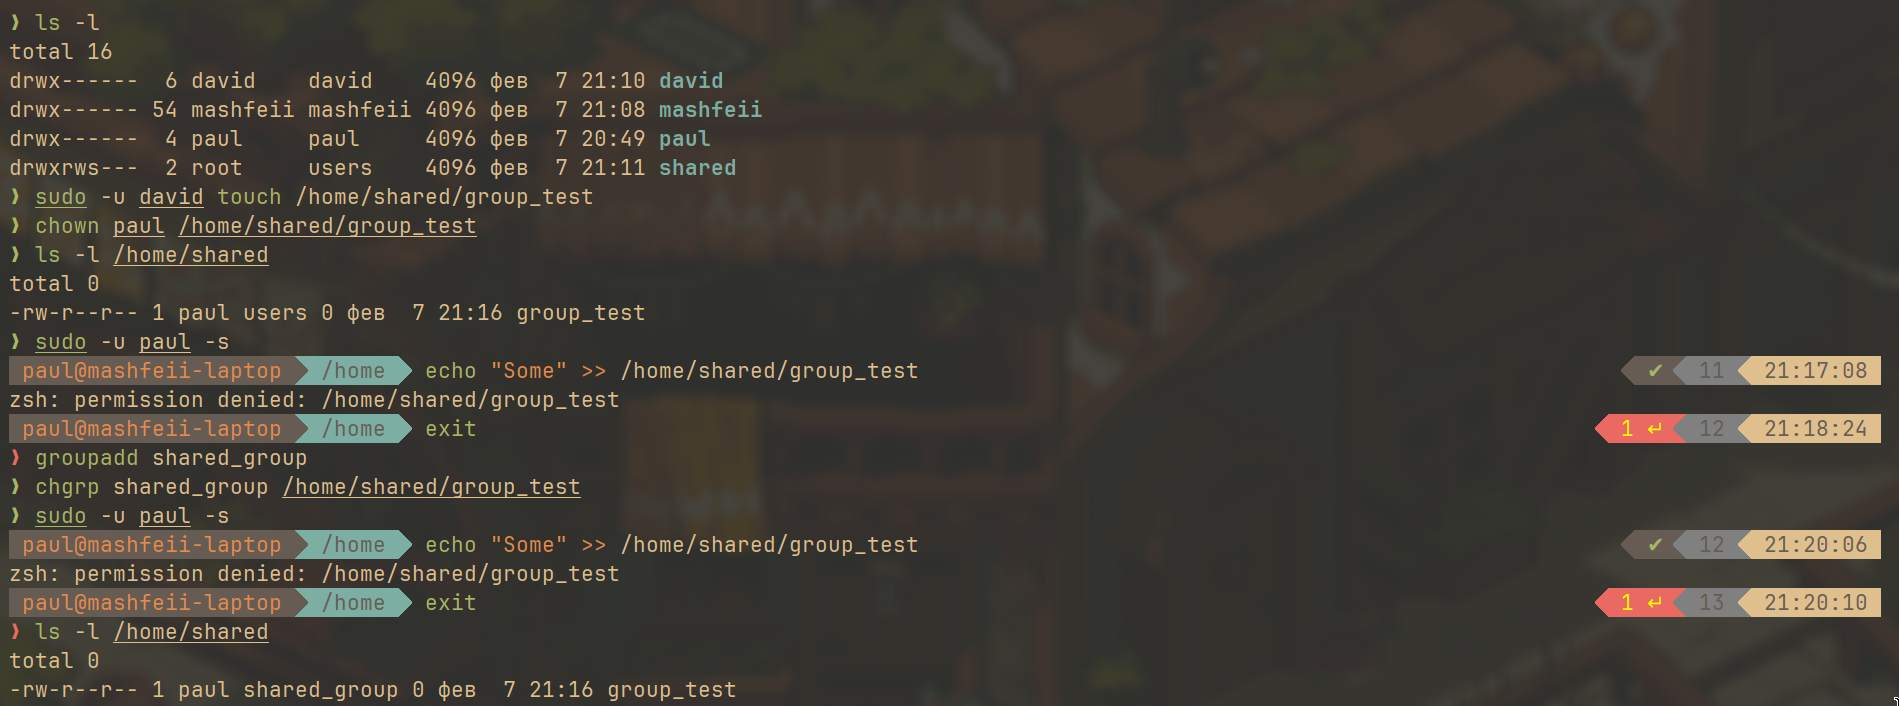
\includegraphics[width=460pt]{03_01.jpg}
\newline

Here are the following sequence of commands:

\begin{enumerate}
	\item Log into as root using \codeword{sudo su}
	\item Check the permissions for \codeword{/home/shared} directory
	\item Create a new file as \codeword{david}, which is in \codeword{users} group
	\item Change the owner to \codeword{paul}, which is not in \codeword{users} group
	\item Try to modify the file as \codeword{paul}
	\item Create new group named \codeword{shared_group} and change \codeword{/home/shared/group_test} file's group to it
	\item Again, try to modify the file as \codeword{paul}
\end{enumerate}

Since the folder \codeword{/home/shared} belongs to \codeword{users} group, \codeword{paul} has no permissions to it according to the first output from \codeword{ls -l /home}, so \codeword{paul} cannot neither access the directory nor modify the file in it.
Changing the file's group to another does not change anything in access, since the directory is still unaccessible for
\codeword{paul}. \\ 

Perhaps the task was supposed to access the folder for users outside the \codeword{users} group, but I continued to complete this task based on lab work.

\section{Text filtering editors}

\subsection{Error and Warning messages}
\noindent

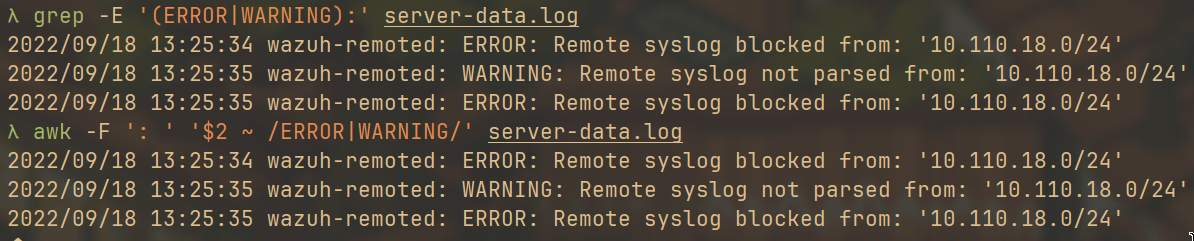
\includegraphics[width=460pt]{3_2-1.jpg}
\newline

Here, for \codeword{grep} we extend the regexp with \codeword{-E} flag to capture the desired lines.

For \codeword{awk} we specify \codeword{': '} as field separator, take the second field and look for \codeword{ERROR} or \codeword{WARNING} in it.

\subsection{Exclude INFO messages}
\noindent

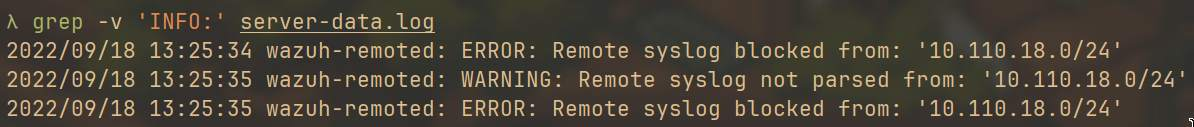
\includegraphics[width=460pt]{3_2-2.jpg}
\newline

Flag \codeword{-v} is used to exclude lines matching the regexp (which contains \codeword{INFO} string).

\subsection{Count ERORR messages}
\noindent

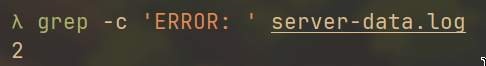
\includegraphics[width=300pt]{3_2-3.jpg}
\newline

With flag \codeword{-c} we count the number of matching lines.

\subsection{Hide IP addresses}
\label{sec:strict}
\noindent

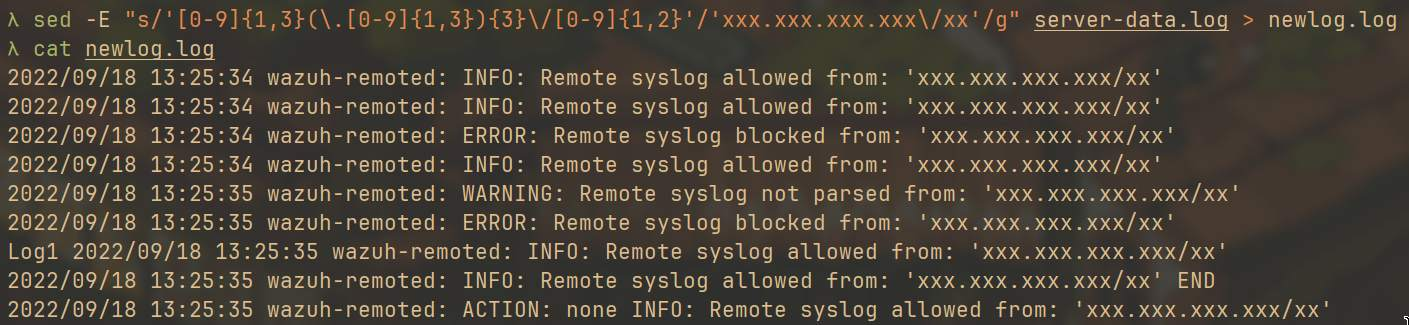
\includegraphics[width=460pt]{3_2-4.jpg}
\newline

With \codeword{sed} we can efficiently filter the input stream from input file, find all the appropriate character sequences (four groups of one to three digits and one of the same group after the hyphen) and replace them with the required text.

\subsection{Strict Regexp}

\noindent

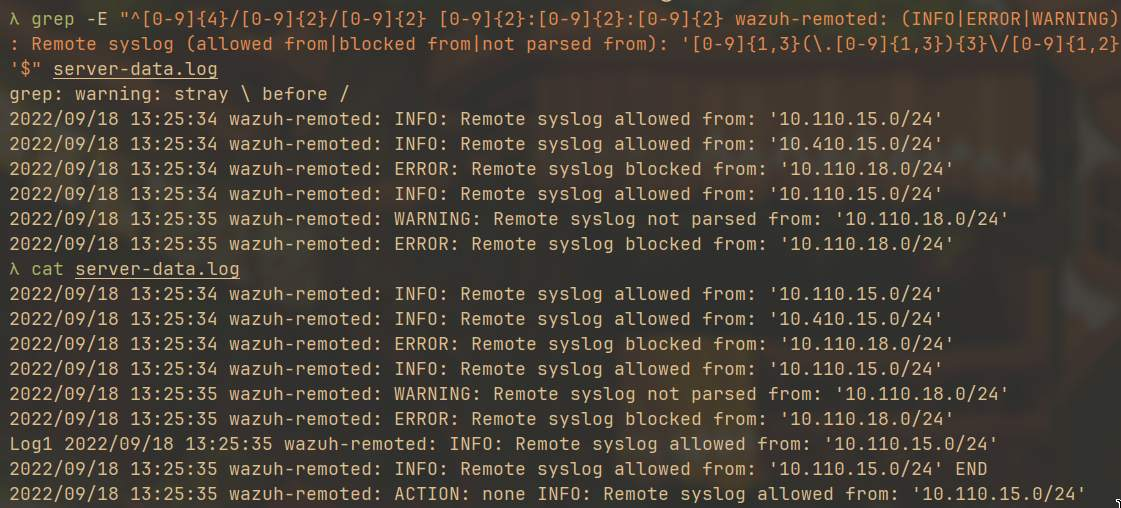
\includegraphics[width=460pt]{3_2-5.jpg}
\newline

I have divided the regular expression into the following groups (not explicitly highlighted inside the expression):

\begin{enumerate}
	\item \codeword{^} - start of the line
	\item \codeword{[0-9]{4}/[0-9]{2}/[0-9]{2}} - date in format \codeword{YYYY/MM/DD}, where \codeword{YYYY} is 4 digits, \codeword{MM} is 2 digits and \codeword{DD} is 2 digits
	\item \codeword{[0-9]{2}:[0-9]{2}:[0-9]{2}} - time in format \codeword{HH:MM:SS}, where each part is 2 digits
	\item \codeword{wazuh-remoted: } - strict character matching
	\item \codeword{(INFO|ERROR|WARNING)} - one of the possible variants
	\item \codeword{: Remote syslog } - strict character matching
	\item \codeword{(allowed from|blocked from|not parsed from): } - one of the possible variants + strict separator/character matching
  \item \codeword{'[0-9]{1,3}(\.[0-9]{1,3}){3}\/[0-9]{1,2}'} - IP address, same as in \hyperref[sec:strict]{point 2.4}
  \item \codeword{$} - end of the line
\end{enumerate}

\section{Bonus}
\noindent

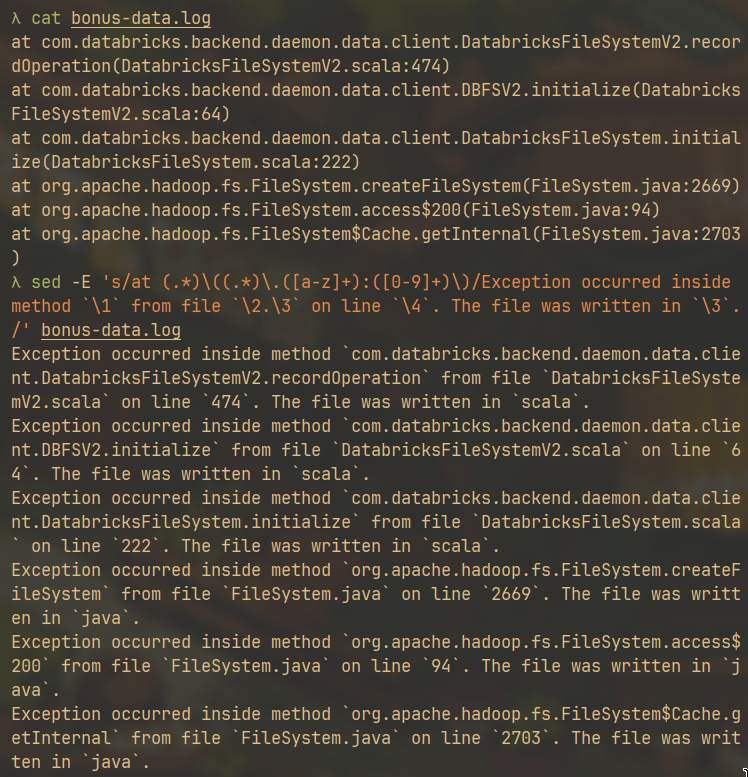
\includegraphics[width=460pt]{3_bon-1.jpg}
\newline

I have divided the regular expression into the following groups:

\begin{enumerate}
  \item \codeword{at} - string character matching
  \item \codeword{(.*)} - first group, any character 0 or more times for method name
  \item \codeword{(.*)\.([a-z]+)} - second group and third group divided by a dot, any characters for file name, lowercase characters (at least 1) for file extension
  \item \codeword{:} - strict character matching for separator
  \item \codeword{([0-9]+)} - fourth group, one or more digits for line number
  \item the groups from the second to the last are surrounded by parentheses \codeword{\(}, \codeword{\)}
\end{enumerate}

\end{document}
